\documentclass[10pt,a4paper,french]{article}
\usepackage{babel}
\usepackage[utf8]{inputenc}
\usepackage[T1]{fontenc}
\usepackage{../latex/clovisai}

\usepackage{pgf-umlcd}

\makeindex
\makeglossaries

\newacronym{uml}{UML}{Unified Modeling Language}

\begin{document}

\title{\glsdesc{uml}}
\author{Ivan Canet}
\maketitle

\begin{abstract} % ARTICLE ONLY
Ceci est l'introduction du document.
\end{abstract}

\tableofcontents

\section{Diagramme de classe}

\subsection{Classes}

\subsubsection{Classe normale}

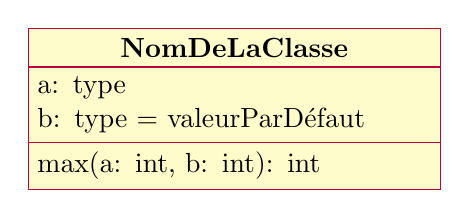
\begin{tikzpicture}
\begin{class}{NomDeLaClasse}{0,0}
	\attribute{a: type}
	\attribute{b: type = valeurParDéfaut}
	\operation{max(a: int, b: int): int}
\end{class}
\end{tikzpicture}

\subsubsection{Classe abstraite}

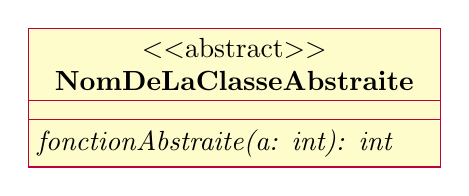
\begin{tikzpicture}
\begin{abstractclass}{NomDeLaClasseAbstraite}{0,0}
	\operation[0]{fonctionAbstraite(a: int): int}
\end{abstractclass}
\end{tikzpicture}

\subsubsection{Interface}

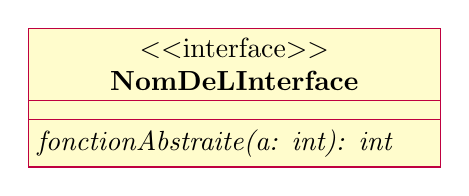
\begin{tikzpicture}
\begin{interface}{NomDeLInterface}{0,0}
	\operation[0]{fonctionAbstraite(a: int): int}
\end{interface}
\end{tikzpicture}

\subsection{Visibilités}

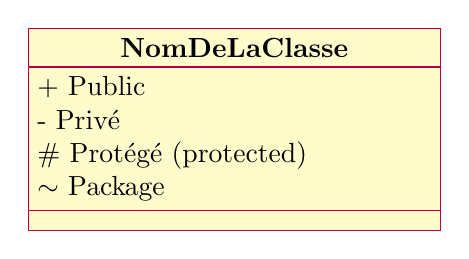
\begin{tikzpicture}
\begin{class}{NomDeLaClasse}{0,0}
	\attribute{+ Public}
	\attribute{- Privé}
	\attribute{\# Protégé (protected)}
	\attribute{$\sim$ Package}
\end{class}
\end{tikzpicture}

\subsection{Relations}

\subsubsection{Héritage}

On utilise une flèche creuse pour l'héritage, en pointillés pour une relation d'implémentation (avec une interface).

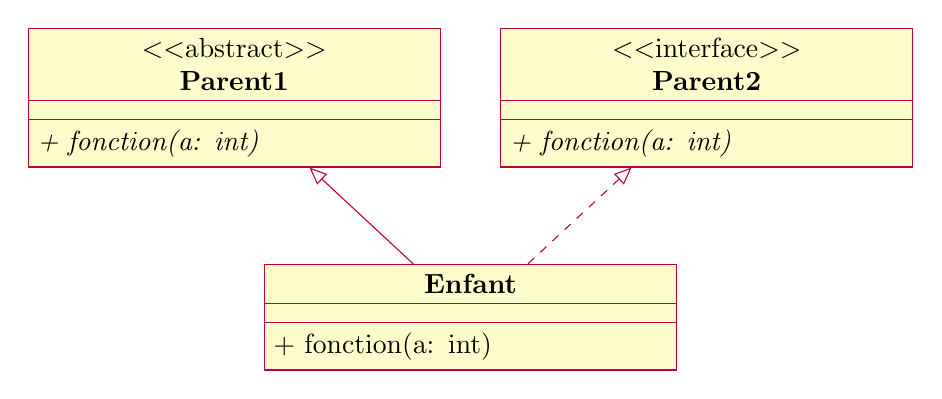
\begin{tikzpicture}
\begin{abstractclass}{Parent1}{0,0}
	\operation[0]{+ fonction(a: int)}
\end{abstractclass}

\begin{interface}{Parent2}{6,0}
	\operation[0]{+ fonction(a: int)}
\end{interface}

\begin{class}{Enfant}{3,-3}
	\inherit{Parent1}
	\implement{Parent2}
	\operation{+ fonction(a: int)}
\end{class}
\end{tikzpicture}

\subsubsection{Association, agrégation, composition}

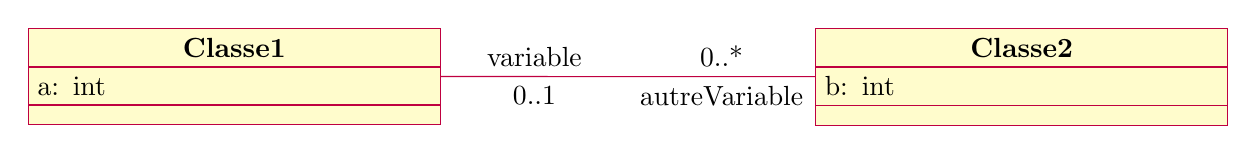
\begin{tikzpicture}
\begin{class}{Classe1}{0,0}
	\attribute{a: int}
\end{class}

\begin{class}{Classe2}{10,0}
	\attribute{b: int}
\end{class}

\association{Classe1}{variable}{0..1}{Classe2}{0..*}{autreVariable}
\end{tikzpicture}

On peut aussi utiliser des associations unidirectionnelles :

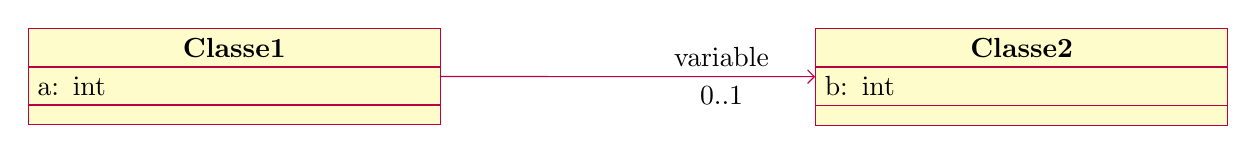
\begin{tikzpicture}
\begin{class}{Classe1}{0,0}
	\attribute{a: int}
\end{class}

\begin{class}{Classe2}{10,0}
	\attribute{b: int}
\end{class}

\unidirectionalAssociation{Classe1}{variable}{0..1}{Classe2}
\end{tikzpicture}

Une agrégation représente que l'élément principal est un agrégat (un regroupement) d'un ou plusieurs éléments. Ces éléments peuvent fonctionner indépendamment : par exemple, un train est un agrégat de wagons, mais chaque wagon peut exister de lui-même et être associé à une autre locomotive, etc.

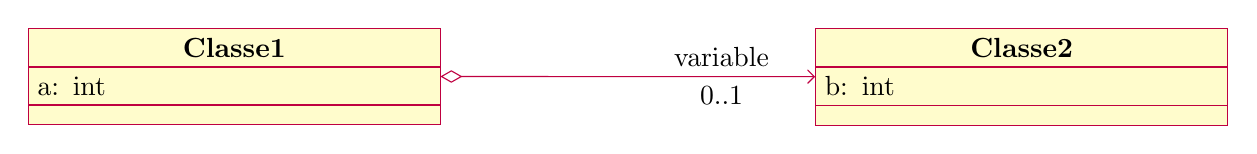
\begin{tikzpicture}
\begin{class}{Classe1}{0,0}
	\attribute{a: int}
\end{class}

\begin{class}{Classe2}{10,0}
	\attribute{b: int}
\end{class}

\aggregation{Classe1}{variable}{0..1}{Classe2}
\end{tikzpicture}

Une composition est similaire à une agrégation, sauf qu'elle est plus `forte' : cette fois, l'élément majeur est `composé' d'autres éléments, qui ne peuvent pas exister seuls : par exemple, une maison est composé d'un certain nombre de pièces ; une maison a forcément des pièces, et une pièce ne peut pas exister en dehors d'une maison !

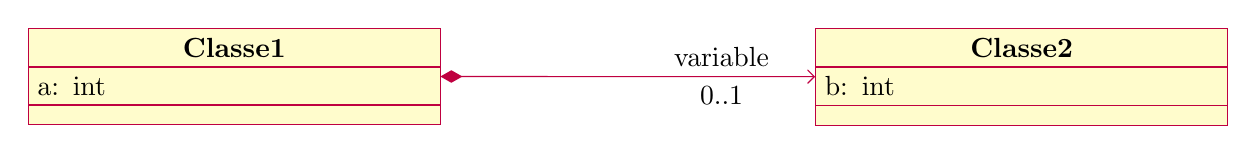
\begin{tikzpicture}
\begin{class}{Classe1}{0,0}
	\attribute{a: int}
\end{class}

\begin{class}{Classe2}{10,0}
	\attribute{b: int}
\end{class}

\composition{Classe1}{variable}{0..1}{Classe2}
\end{tikzpicture}

\appendix % Annexes, ARTICLE & BOOK

%\bibliography{•} % THE .BIB FILE HERE, WITHOUT THE EXTENSION
\printindex
\printglossaries

\end{document}
